\documentclass[12pt,a4paper]{report}
\usepackage[utf8]{inputenc}
\usepackage[spanish]{babel}
\usepackage{amsmath}
\usepackage{amsfonts}
\usepackage{amssymb}
\usepackage{graphicx}
\graphicspath{ {images/} }
\usepackage{color}

\definecolor{miverde}{rgb}{0,0.6,0}
\definecolor{migris}{rgb}{0.5,0.5,0.5}
\definecolor{mimalva}{rgb}{0.58,0,0.82}
\usepackage{listings}%Para insertar codigo de programacion
\lstset{ %
  backgroundcolor=\color{white},   % Indica el color de fondo; necesita que se añada \usepackage{color} o \usepackage{xcolor}
  basicstyle=\footnotesize,        % Fija el tamaño del tipo de letra utilizado para el código
  breakatwhitespace=false,         % Activarlo para que los saltos automáticos solo se apliquen en los espacios en blanco
  breaklines=true,                 % Activa el salto de línea automático
  captionpos=b,                    % Establece la posición de la leyenda del cuadro de código
  %commentstyle=\color{miverde},    % Estilo de los comentarios
  deletekeywords={...},            % Si se quiere eliminar palabras clave del lenguaje
  escapeinside={\%*}{*)},          % Si quieres incorporar LaTeX dentro del propio código
  extendedchars=true,              % Permite utilizar caracteres extendidos no-ASCII; solo funciona para codificaciones de 8-bits; para UTF-8 no funciona. En xelatex necesita estar a true para que funcione.
  frame=single,	                   % Añade un marco al código
  keepspaces=true,                 % Mantiene los espacios en el texto. Es útil para mantener la indentación del código(puede necesitar columns=flexible).
  keywordstyle=\color{blue},       % estilo de las palabras clave
  language=csh,                 % El lenguaje del código
  otherkeywords={*,...},           % Si se quieren añadir otras palabras clave al lenguaje
  numbers=left,                    % Posición de los números de línea (none, left, right).
  numbersep=5pt,                   % Distancia de los números de línea al código
  numberstyle=\small\color{migris}, % Estilo para los números de línea
  rulecolor=\color{black},         % Si no se activa, el color del marco puede cambiar en los saltos de línea entre textos que sea de otro color, por ejemplo, los comentarios, que están en verde en este ejemplo
  showspaces=false,                % Si se activa, muestra los espacios con guiones bajos; sustituye a 'showstringspaces'
  showstringspaces=false,          % subraya solamente los espacios que estén en una cadena de esto
  showtabs=false,                  % muestra las tabulaciones que existan en cadenas de texto con guión bajo
  stepnumber=1,                    % Muestra solamente los números de línea que corresponden a cada salto. En este caso: 1,3,5,...
  stringstyle=\color{mimalva},     % Estilo de las cadenas de texto
  tabsize=2,	                   % Establece el salto de las tabulaciones a 2 espacios
  title=\lstname                   % muestra el nombre de los ficheros incluidos al utilizar \lstinputlisting; también se puede utilizar en el parámetro caption
}
\author{Elaborado por:\\\\Rivera Negrete Manuel Armando}
\date{28 de Junio del 2018}
\title{Universidad Nacional Autónoma de México\\Programa de Tenología en Cómputo\\Lo que siempre quisiste saber de C\# y nunca te atreviste a preguntar}

\begin{document}
\maketitle
\tableofcontents
\cleardoublepage
\part*{¿Por qué aprender C\#?}

\part{C\# Básico}

\chapter{La arquitectura .NET}
\section{C\# y su lugar dentro de .NET}
C\# (leído <<C sharp>>) es un lenguaje de programación orientado a objetos desarrollado y estandarizado por Microsoft como partes de su plataforma .NET. Aunque esta plataforma permite desarrollar aplicaciones en otros lenguajes de programación, C\# ha sido creado específicamente para .NET, adecuando todas sus estructuras a las características y capacidades de dicha plataforma.\\.NET es un framework de Microsoft que hace un énfasis en el desarrollo sencillo de aplicaciones, independencia de hardware y transparencia de redes. Es una implementación de Common Language Infraestructure (Estandar CLI). Un Framework es un esquema (un esqueleto, un patrón) para el desarrollo y/o la implementación de una aplicación.
%Á á, É é, Í í,Ó ó,Ú ú,Ü ü,Ñ ñ, ¿, ¡ ``
\section{Common Language Runtime}
El Common Language Runtime o CLR es un entorno de ejecución que ejecuta el código y proporciona servicios que facilitan el proceso de desarrollo de los programas que corren sobre la plataforma Microsoft .NET.\\Los compiladores y las herramientas exponen la funcionalidad del tiempo de ejecución del idioma común y le permiten escribir código que se beneficia de este entorno de ejecución administrada. El código que desarrolla con un compilador de lenguaje que se dirige al tiempo de ejecución se denomina código administrado; se beneficia de características tales como la integración entre idiomas, manejo de excepciones entre idiomas, seguridad mejorada, soporte de versiones e implementación, un modelo simplificado para la interacción de componentes y servicios de depuración y creación de perfiles. Para enternder el proceso de compilación en C\# es necesario definir algunos conceptos:\\Compilación: La tarea de compilar se refiere al proceso de traducción del código fuente a código entendible por la computadora, entendiéndose por código fuente las líneas de código que se han escrito en un lenguaje de programación, en este caso un lenguaje de programación de alto nivel.\\Código Máquina: Es el sistema de códigos directamente interpretable por un circuito microprogramable, como el microprocesador de una computadora, es decir, es un lenguage que entiende la computadora.\\ByteCode: Es un código intermedio más abstracto que el código máquina. Habitualmente es tratado como un archivo binario que contiene un programa ejecutable similar a un módulo objeto, que es un archivo binario producido por el compilador cuyo contenido es el código objeto o código máquina.\\
\section{Microsoft Intermediate Language}
MSIL significa Microsoft Intermediate Language. Podemos llamarlo Lenguaje Intermedio (IL) o Lenguaje Intermedio Común (CIL). Durante el tiempo de compilación, el compilador convierte el código fuente en Microsoft Intermediate Language (MSIL). Microsoft Intermediate Language (MSIL) es un conjunto de instrucciones independiente de la CPU que se puede convertir de manera eficiente al código nativo. Durante el tiempo de ejecución, el compilador Just In Time (JIT) de Common Language Runtime (CLR) convierte el código de Microsoft Intermediate Language (MSIL) en código nativo al sistema operativo.\\El código fuente escrito en C\# se compila en un lenguaje intermedio (IL) que guarda conformidad con la especificación de CLI. El código y los recursos IL, como mapas de bits y cadenas, se almacenan en disco en un archivo ejecutable denominado ensamblado, normalmente con la extensión .exe o .dll. Un ensamblado contiene un manifiesto que proporciona información sobre los tipos, la versión, la referencia cultural y los requisitos de seguridad del ensamblado.\\Cuando se ejecuta el programa de C\#, el ensamblado se carga en el CLR, el cual podría realizar diversas acciones en función de la información en el manifiesto. Luego, si se cumplen los requisitos de seguridad, el CLR realiza la compilación Just in time (JIT) para convertir el código IL en instrucciones máquina nativas. El CLR también proporciona otros servicios relacionados con la recolección de elementos no utilizados, el control de excepciones y la administración de recursos. El código que se ejecuta en el CLR se conoce a veces como "código administrado", a diferencia del "código no administrado" que se compila en lenguaje de máquina nativo destinado a un sistema específico. En el siguiente diagrama se ilustran las relaciones de tiempo de compilación y tiempo de ejecución de archivos de código fuente de C\#, las bibliotecas de clases de .NET Framework, los ensamblados y el CLR.\\Ninguno de los compiladores que generan código para la plataforma .NET produce código máquina para CPUs x86 ni para ningún otro tipo de CPU concreta, sino que generan código escrito en el lenguaje intermedio conocido como Microsoft Intermediate Lenguage (MSIL) El CLR da a las aplicaciones la sensación de que se están ejecutando sobre una máquina virtual, y precisamente MSIL es el código máquina de esa máquina virtual. Es decir, MSIL es el único código que es capaz de interpretar el CLR, y por tanto cuando se dice que un compilador genera código para la plataforma .NET lo que se está diciendo es que genera MSIL.\\MSIL ha sido creado por Microsoft tras consultar a numerosos especialistas en la escritura de compiladores y lenguajes tanto del mundo académico como empresarial. Es un lenguaje de un nivel de abstracción mucho más alto que el de la mayoría de los códigos máquina de las CPUs existentes, e incluye instrucciones que permiten trabajar directamente con objetos (crearlos, destruirlos, inicializarlos, llamar a métodos virtuales, etc.), tablas y excepciones (lanzarlas, capturarlas y tratarlas).
\begin{figure}[hbtp]
\centering
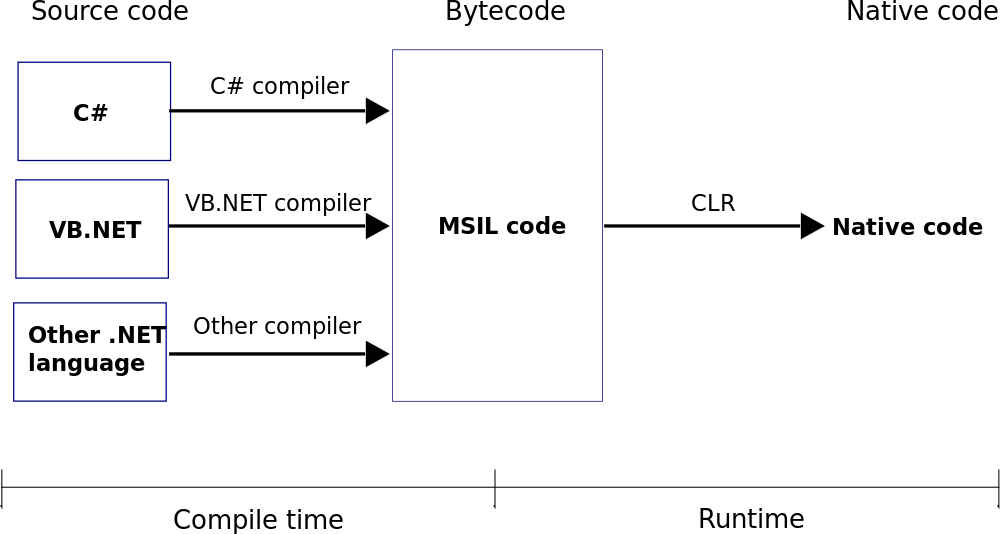
\includegraphics[width=15cm]{Csh_Imagenes/Compilacion.png}
\caption{Compilación en C\#}
\end{figure}
\section{Assemblies}
Los assemblies son los bloques de construcción de las aplicaciones del framework .NET. Un assembly es una colección de tipos y recursos que están construidos para trabajar en conjunto y formar la unidad lógica de la funcionalidad del programa.\\Todos los tipos en .NET Framework deben existir en assemblies; el tiempo de ejecución de idioma común no admite tipos fuera de ensamblados. Cada vez que crea una aplicación de Microsoft Windows, un servicio de Windows, una biblioteca de clases u otra aplicación con Visual Basic .NET, está creando un solo assembly. Cada assembly se almacena como un archivo .exe o .dll.\\Aunque es técnicamente posible crear assemblies que abarquen múltiples archivos, no es probable que use esta tecnología en la mayoría de las situaciones.\\.NET Framework usa assemblies como la unidad fundamental para varios propósitos:\\•Seguridad\\•Tipo de identidad\\•Versiones\\•Desarrollo

\chapter{Introducción a Visual Studio 2017 y C\# }
\section{Características de C\#}
C\# es un lenguaje de programación orientado a objetos, al ser posterior a C++ y Java. los lenguajes de programación orientados a objetos más conocidos hasta entonces, C\# combina y mejora gran parte de las características más interesantes de ambos lenguajes. Por tanto, un programador que conozca C\# a fondo no tendrá problemas para programar tanto en C++ como en Java, sus anteccesores.\\El nombre fue inspirado por la notación musical '\#' (llamada sostenido, en inglés Sharp) que indica que la nota es de un tono más alto. Se puede utilizar C\# para crear aplicaciones cliente de Windows, servicios Web XML, componentes distribuidos, aplicaciones cliente-servidor, aplicaciones de base de datos, y mucho, mucho más.\\Para poder crear programas en C\# y ejecutarlos posteriormente, es necesario tener instalado en el PC los siguientes paquetes:\\\\\textbf{.NET Framework SDK:} Es el kit de desarrollo e incluye un compilador de línea de C\# y bibliotecas que contienen una amplia colección de clases previamente definidas que podemos utilizar en nuestras aplicaciones; es decir, contiene todo lo necesario para poder crear y compilar nuestros programas.\\\textbf{.NET Framework Redistributable Package: } Permite la ejecución de programas creados en C\#. Esto es necesario porque la compilación de C\# no genera, como habitualmente para otros lenguajes, código máquina, sino un código escrito en un lenguaje propio de Microsoft: MSIL (Microsoft Intermediate Language). El CLR (Common Language Runtime) es el núcleo de la plataforma .NET y se encarga de gestionar la ejecución de los programas escritos en MSIL, ambos se pueden descargar gratuitamente desde la página web de la Red de Desarrolladores para Microsoft (Microsoft Developers Network) :\\ \textbf{https://www.microsoft.com/es-mx/download}\\\\También pueden crearse programas mediante la herramienta Visual Studio(Incluye en su instalación dichos paquetes), que ofrece un interfaz gráfico muy amigable y cómodo de utilizar, esta herramienta cuenta con una versión de paga y una gratuita (Community) y se puede descargar directamente desde la página oficial.\\\textbf{https://visualstudio.microsoft.com/es/}\\\\En la figura 2.2 se muestra un menú de paquetes complementarios que podemos descargar, si sólo queremos desarrollar en C\# basta con seleccionar los primeros dos paquetes.
\begin{figure}[hbtp]
\centering

\includegraphics[width=16cm]{Csh_Imagenes/Descarga1.png}
\caption{Página oficial para descargar Visual Studio}
\end{figure}
\begin{figure}[hbtp]
\centering
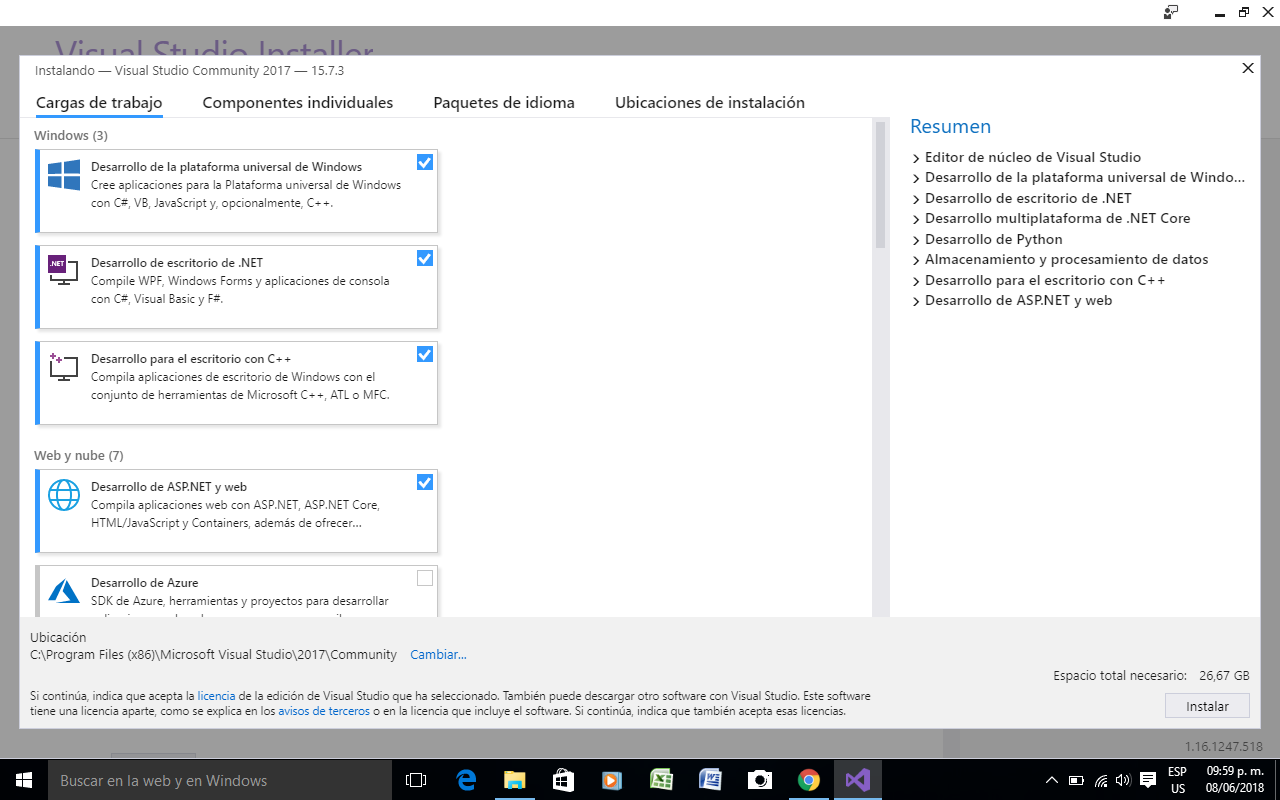
\includegraphics[width=16cm]{Csh_Imagenes/Instalacion.png}
\caption{}
\end{figure}
\section{Estructura de un programa}
Al abrir Visual Studio en la parte superior podemos observar un menú, para empezar un nuevo proyecto hacemos clic en la pestaña de Archivo, posteriormente seleccionamos la opción de nuevo y después proyecto, también podemos presionar la combinación de teclas Ctrl+Mayus+N. Se nos abrirá una ventana en la cual seleccionaremos la opción << Aplicacion de Consola >> y procedemos a darle un nombre a nuestro proyecto y damos click en aceptar. Ver las figuras 2.3 y 2.4.\\
\begin{figure}[hbtp]
\centering
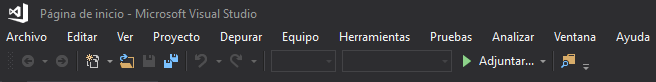
\includegraphics[width=16cm]{Csh_Imagenes/Menu_sup.PNG}
\caption{Menú superior en Visual Studio}
\end{figure}
\begin{figure}[hbtp]
\centering
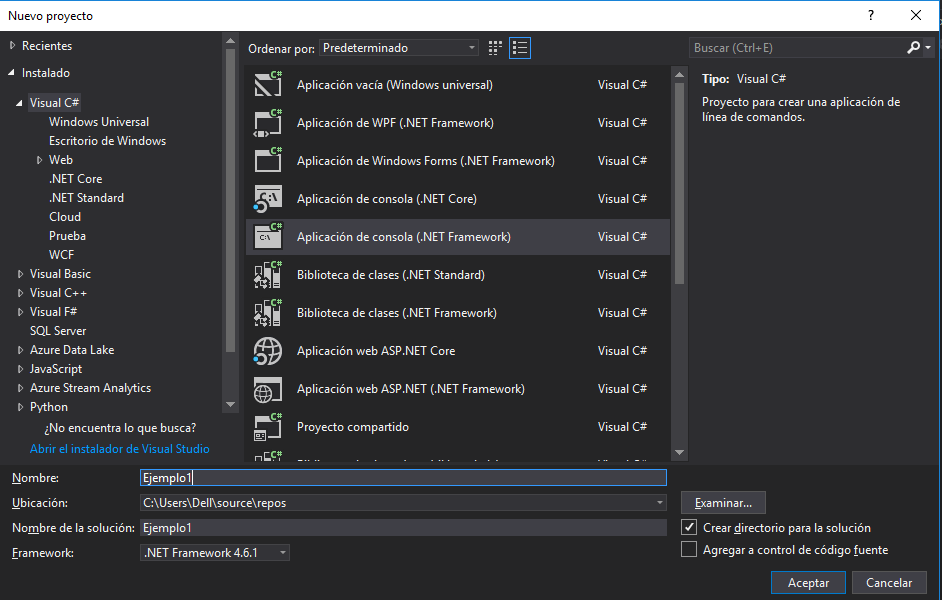
\includegraphics[width=16cm]{Csh_Imagenes/ConsoleApp.PNG}
\caption{}
\end{figure}
Para crear un proyecto sin Visual Studio necesitamos un editor de texto plano y los paquetes antes mencionados. Creamos una carpeta en el escrito llamada csharp, abrimos el block de notas y en este escribimos el código del ejemplo 1 con la extension \textit{.cs} y los guardamos dentro de la carpeta. Para poder compilar y ejecutar este programa necesitamos tener el comando \textit{csc} (el compilador de C\# incluido en la plataforma .NET) accesible. Para ello hay que modificar la variable de entorno Path, que contiene las carpetas en las que el sistema busca los programas a los que se invoca desde la línea de comandos. El proceso es el siguiente:\\\\\textbf{1.-} Buscar el lugar donde está instalada nuestra versión de .NET El Lugar por defecto es en una carpeta de la forma vXXXXX (donde XXXXX representa el número de versión de .NET que hemos instalado) que puede encontrarse en:\\\textbf{C:\textbackslash Windows\textbackslash Microsoft.NET\textbackslash Framework\textbackslash vX.X.XXXXX}\\\\\textbf{2.-} Abrir la cmd, esto se puede hacer abriendo el explorador y poner cmd o presionar la combinacion de las teclas Windows + R y escribir cmd. En la ventana de comandos escribir:\\\textbf{path=\%path\%;C:\textbackslash Windows\textbackslash Microsoft.NET\textbackslash Framework\textbackslash vX.X.XXXXX}.\\El comando \textit{csc} ya debe estar accesible desde la línea de comandos.\\\\C\# es un lenguaje orientado a objetos. En cualquier programa en C\# debe existir al menos una clase que contenga un método llamado \textbf{Main}. Este método constituye lo que se denomina punto de entrada, y define por dónde ha de comenzar a ejecutarse la aplicación: la primera instrucción ejecutada será la primera instrucción del método \textbf{Main}.\\El siguiente ejemplo muestra el programa más simple que puede crearse en C\#.\\\\

\textbf{Ejemplo 2.1}
\begin{lstlisting}
using System;
//Usamos el espacio de nombres System
class Ejemplo1 {
	static void Main() {
	
	}
}
\end{lstlisting}
Para crear una clase hay que escribir la palabra reservada \textbf{class} seguida del nombre que queremos darle. A continuación entre llaves, aparecerán los métodos y atributos de dicha clase. En este ejemplo hemos creado la clase \textit{Ejemplo 2.1}, que no incluye ningún atributo y contiene un solo método, de nombre \textbf{Main}. Como hemos dicho, todo programa en C\# debe contener al menos una clase con un método llamado \textbf{Main}.\\\\Es importante aclarar que C\# se distinguen las mayúsculas de las minúsculas, algo que no curre en todos los lenguajes de programación. Así, el punto de entrada ha de llamarse \textit{Main} y no \textit{main} o \textit{MAIN} o ninguna otra variante.\\\\Como para cualquier otro método existen varias alternativas válidas oara crear la declaración del método \textbf{Main}. Algunas son: \\\\\textit{public static int Main()\\public static void Main(string[] args)\\static int Main(string[] args)}\\\\La palabra \textbf{public} indica que el método es público, es decir, puede ser utilizado por otra clase (si no se pone nada, se considerará privado por defecto). La palabra \textbf{static} indica que que el método está asociado a la clase a la que pertenece y no a los objetos que se creen de dicha clase. En tercer lugar, aparece el tipo de la información que devuelve el método: \textbf{int} indica que devuelve un dato de tipo entero; \textbf{void}  indica que no se devuelve ningún valor. A continuación del nombre del método, que para el punto de entrada siempre es \textbf{Main}, aparecen entre paréntesis los argumentos o datos de entrada de este método, es decir, la información de la partida que requiere. Esta sección puede estar vacía.\\\\Por el momento dado los escasos conocimientos que aún tenemos, será suficiente con que el punto de entrada sea estático, no tenga argumentos y no devuelva ningún valor, tal y como se declaró en el ejemplo.
\section{Compilación y ejecución}
La compilación y ejecución usando Visual Studio resulta ser muy sencilla sin embrago se explicará el proceso con dicha herramienta y sin ella.\\Para compilar nos vamos al menú que se encuentra en la parte superior de la ventana de C\# y damos click en la pestaña donde dice Compilar, posteriormente se nos abrirá un menú en el cual seleccionaremos la opción de compilar solución. Al hacer dicho paso en la parte inferior aparecerá otra ventana conocida como la ventana de salida o de output donde se nos informará de todos los errores en nuestro programa antes de ejecutarlo. Una vez compilado nuestro programa nos vamos a la ventana superior y damos click en la pestaña donde dice depurar, al abrirse el menú seleccionamos la opción de iniciar sin depurar y se nos abrirá la ventana de comandos con nuestro programa en ejecución.\\Para compilar un programa sin Visual Studio nos vamos a la carpeta csharp creada en la sección pasada desde la cmd, para hacer esto abrimos la ventana de comandos y escribimos \textbf{cd c:\textbackslash csharp} y pulsamos intro, despues escribimos \textbf{csc Ejemplo1.cs} si sólo arroja un mensaje en el que nos indique la versión del compilador que se está utilizando, así como la version del Framework que está instalada significa que el código ha sido compilado con éxito, para ejecutar nuestro programa escribimos el nombre de éste sin la extensión .cs.


\chapter{Tipos predefinidos y control de flujo}
En este capitulo se mostrará cómo se utilizan datos de diferentes tipos básicos dentro de un programa y qué tipo de operaciones pueden realizarse con ellos.\\Normalmente, los programas sencillos necesitan de datos muy sencillos, pero los que conocemos hasta ahora son insuficientes. Por ejemplo, no podríamos plantearnos un programa que multiplique dos números enteros.\\\\Para manejar datos de tipos básicos cono enteros o reales, necesitamos dos cosas: poder almacenar esos datos en algún sitio, para lo que se utilizan variables, y poder manipular esos datos, para lo que necesitamos los operadores. Veremos a continuación qué tipos de datos tenemos disponibles en C\# y cuál es el conjunto de operadores que nos va a permitir transformar y operar con dichos datos.
\section{Tipos predefinidos de C\#}
El concepto de dato está relacionado con las operaciones que se pueden realizar sobre él. Un tipo de dato queda definido como un conjunto de valores que tienen asociadas una serie de operaciones para crearlos y manipularlos.\\\\En el ordenador cada tipo de datos se representa de una forma diferente. Una tabla parcial de los tipos que pueden manejarse en C\# se muestra en la figura 3.1
\begin{figure}[hbtp]
\centering
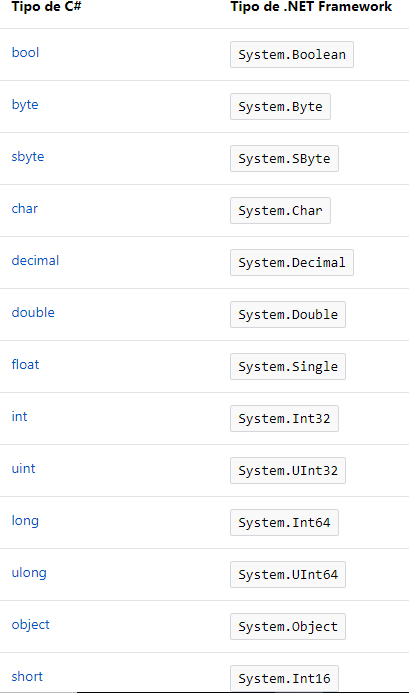
\includegraphics[width=8cm]{Csh_Imagenes/Tabla_Tipos.PNG}
\caption{Resumen del sistema de Tipos de C\#}
\end{figure}
\begin{figure}[hbtp]
\centering
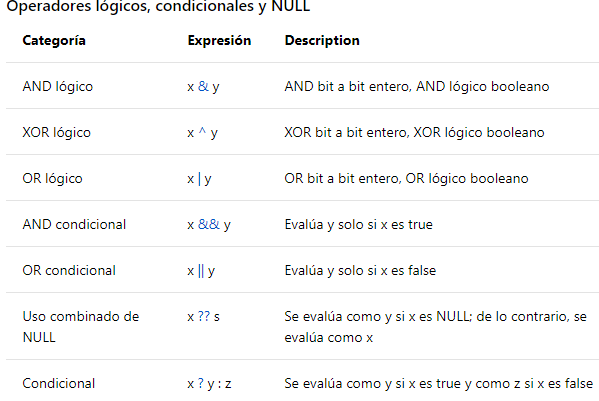
\includegraphics[width=16cm]{Csh_Imagenes/op_condicionales.PNG}
\caption{Operadores lógicos, condicionales y NULL}
\end{figure}
\begin{figure}[hbtp]
\centering
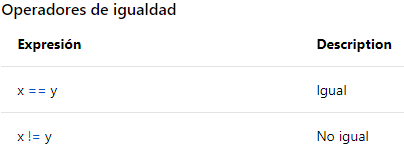
\includegraphics[width=16cm]{Csh_Imagenes/op_igualdad.PNG}
\caption{Operadores de igualdad}
\end{figure}
\begin{figure}[hbtp]
\centering
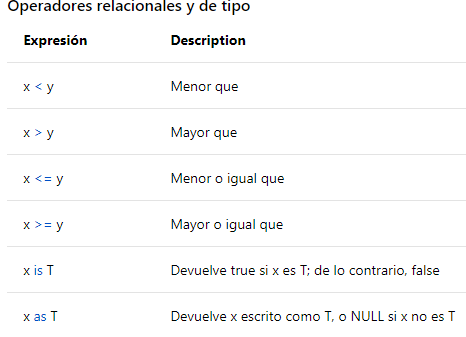
\includegraphics[width=16cm]{Csh_Imagenes/op_relacionales.PNG}
\caption{Operadores relacionales y de tipo}
\end{figure}

El nombre del tipo y la clase donde se define son, en realidad, la misma cosa. Es decir, el nombre del tipo es simplemente un alias y podemos utilizar indistintamente una u otro.\\\\Para aplicaciones grandes que manejan un gran volumen de datos es necesario optimizar el espacio que ocupan esos datos, ajustando lo máximo posible el tipo de las variables a los posibles valores que éstas vayan a almacenar.

\section{Tipos de referencia}
Hay dos clases de tipos en C\#: tipos de referencia y tipos de valor. Las variables de tipos de referencia almacenan referencias en sus datos (objetos), mientras que las variables de tipos de valor contienen directamente los datos. Con los tipos de referencia, dos variables pueden hacer referencia al mismo objeto y, por lo tanto, las operaciones en una variable pueden afectar al objeto al que hace referencia la otra variable. Con los tipos de valor, cada variable tiene su propia copia de los datos, y no es posible que las operaciones en una variable afecten a la otra .\\Las palabras clave siguientes se usan para declarar tipos de referencia:\\\textbf{class}: Palabra reservada para crear clases\\\textbf{Interface}: Una interfaz contiene solo las firmas de métodos, propiedades, eventos o indicadores.\\\textbf{delegate}: La declaración de un tipo delegado es similar a una firma de método. Tiene un valor devuelto y un número cualquiera de parámetros de cualquier tipo.
\section{Sentencias condicionales}
\textbf{Sentencia if}\\La sentencia \textbf{if} permite elegir entre dos alternativas en la función del valor(verdadero o falso) de cierta condición. Si la condición es verdadera, entonces se ejecuta un fragmento de código, y si es falsa, entonces se ejecuta otro distinto (usando la palabra else e indicando otro bloque de código), o no se ejecuta nada (No indicando el bloque de código else).
\textbf{Sintaxis de la instrucción if}.\\La instrucción \textbf{if} debe utilizarse de acuerdo a la siguiente sintaxis:
\begin{lstlisting}
if(<Condicion>)
  <instruccion_if>
else
  <instruccion_else>
\end{lstlisting}
\textbf{Ejemplo 3.1}\\
\begin{lstlisting}
using System;
class Ejemplo_3.1 {
  static void Main() {
    string nombre;  //Esta variable de tipo string guarda el nombre del usuario
    Console.WriteLine("Escribe tu nombre");
    nombre=Console.ReadLine();
    if(nombre == "Armando")
      Console.WriteLine("Bienvenido Armando!");
    else
      Console.WriteLine("Usuario no valido");   

    Console.ReadKey();  //Esta linea es util al ejecturar nuestro programa en Visua Studio para evitar que se cierre la consola inesperadamente.
  }
}
\end{lstlisting}
A menudo nos interesa introducir más de una línea de código en nuestros bloques \textbf{if}, \textbf{else} para esto utilizamos llaves {} en cada bloque.\\
\begin{lstlisting}
if(<Condicion>) {
  <instruccion1_if>
  <instruccion2_if>
  <instruccion3_if>
  <instruccion4_if>
}
else {
  <instruccion1_else>
  <instruccion2_else>
  <instruccion3_else>
}
\end{lstlisting}
En el ejemplo 2 la sentencia \textit{nombre == ``Armando"} regresa un valor y ese valor es \textbf{true} o \textbf{false}\\\\\textbf{La instrucción switch}\\
En ocaciones hay que tomar un gran número e decisiones dependiendo del valor que tiene una determinada expresión. Esto obliga a utilizar una colección de instrucciones \textbf{if} anidadas, tales que todas ellas realizan una comprobación sobre la misma expresión.\\\textbf{Sintaxis de la instrucción switch}\\La instrucción \textbf{switch} debe utilizarse de acuerdo a la siguiente sintaxis:\\
\begin{lstlisting}
switch (<expresion>) {
  case <valor1>: 
    <bloque_de_instrucciones_1>
    break;
  case <valor2>: 
    <bloque_de_instrucciones_2>
    break;
  ......
  case <valorn>: 
    <bloque_de_instrucciones_n>
    break;
  default:
    <bloque_de_instrucciones>
    break;
}
\end{lstlisting}
El significado de esta instrucción es la siguiente: se evalúa \textit{expresión}. Si su valor es \textit{valor1} se ejecuta \textit{bloque de instrucciones 1}, si es \textit{valor2} se ejecuta \textit{bloque de instruciones 2}, y así para el resto de valores especificados. Si no es igual a ninguno de esos valores y se incluye la rama \textbf{default}, se ejecuta \textit{<bloque de instrucciones>}; si no se incluye se pasa directamente a ejecutar la instrucción siguiente al \textbf{switch}.\\Los valores indicados en cada rama del \textbf{switch} han de ser expresiones constantes que produzcan valores de algún tipo básico. No puede haber más de una rama con el mismo valor. Cada bloque de instrucciones de cada rama debe terminar con una instrucción \textbf{break} para indicarle que continúe la ejecución con la siguiente instrucción al \textbf{switch}.
\\\textbf{Ejemplo 3.2}.
\begin{lstlisting}
using System;
class Ejemplo_Switch 
{
    static void Main()
    {
        Console.WriteLine("Cafes: 1=Chico 2=Mediano 3=Grande"); 
        Console.Write("Introduzca el cafe deseado: "); 
        string s = Console.ReadLine(); 
        int n = int.Parse(s); //Esta linea hace un casteo de cadena a un valor entero
        int cost = 0;
        switch(n)
        {
        case 1:
            cost += 25;
            break;
        case 2:
            cost += 50;
            break;
        case 3:
            cost += 75;
            break;
        default:
            Console.WriteLine("Seleccion invalida, Seleccione solo 1, 2, o 3.");
            break;
        }
        if (cost != 0)
        {
            Console.WriteLine("Introduzca {0} pesos.", cost);
        }
        Console.WriteLine("Gracias por su compra.");
    }
}
\end{lstlisting}
%Á á, É é, Í í,Ó ó,Ú ú,Ü ü,Ñ ñ, ¿, ¡ ``
\section{Ciclos de repetición}
\textbf{La instrucción while}\\Permite ejecutar un bloque de instrucciones mientras se cumpla una cierta condición: si la condición es verdadera, entonces se ejecuta el fragmento de código incluido dentro del \textbf{while}, y si es falsa, se salta el bucle y no se ejecuta nada.\\\textbf{Sintaxis de la instrucción while}\\La instrucción while debe utilizarse de acuerdo a la siguiente sintaxis.
\begin{lstlisting}
	while(<condicion>)
		<instrucciones>
\end{lstlisting}
\textbf{Ejemplo 3.3}.
\begin{lstlisting}
using System;
class Ejemplo_While 
{
    static void Main() {
    	int n = 0;
		while (n < 5) {
    		Console.WriteLine(n);
	    	n++;
		}
    }
}
\end{lstlisting}
Este ejemplo imprime los números del 0 al 4, es decir, el código se repite hasta que n sea menor a 5.\\\textbf{El bucle for}\\Un bucle for ejecuta un conjunto de declaraciones un número específico de veces y tiene la sintaxis.\\
\begin{lstlisting}
for(init; condicion; incremento;) {
	<Instrucciones>
}
\end{lstlisting}
Un contador es declarado una vez en \textbf{init}. A continuación, la \textbf{condicion} evalúa el valor del contador y el cuerpo del bucle es ejecutado si la condición es verdadera.\\Después de la ejecución del bucle, la declaración de \textbf{incremento} actualiza el contador, también llamado la variable de control del bucle.\\La condición es evaluada una vez más, y el cuerpo del bucle se repite, sólo deteniéndose cuando la condición se vuelve \textbf{falsa}.\\\textbf{Ejemplo 3.4}
\begin{lstlisting}
using System;
class Ejemplo_for {
	static void Main() {
		for(int x = 10; x < 15; x++) {
			Console.WriteLine("El valor de x es: " + x);		
		}
	}
}
\end{lstlisting}El anterior ejemplo imprime los números del 10 al 14\\En la última sección del \textbf{for} puede ir en lugar de x++ x+=3 o x-=2 dependiendo del interés del programador.\\Las declaraciones \textbf{init} e \textbf{incremento} pueden ser omitidas, si no se requieren, pero recuerda que los puntos y comas son obligatorios.\\\textbf{Ejemplo 3.5}\begin{lstlisting}
using System;
class Ejemplo_for {
	static void Main() {
	int x = 10;
		for(; x < 15; ) {
			Console.WriteLine("El valor de x es: " + x);
			x-=3;		
		}
	}
}
\end{lstlisting}El ciclo \textbf{for(;;){}} es un bucle infinito.\\\\
\textbf{El Bucle do-while}
Un bucle do-while es similar a un bucle \textbf{while}, excepto que un bucle \textbf{do-while} está garantizado a ser ejecutado al menos una vez.\\\\\textbf{Ejemplo 3.6}
\begin{lstlisting}
using System;
class Ejemplo_do_while {
	static void Main() {
	int x = 0;
		do {
			Console.WriteLine("El valor de x es: " + x);
			x++;		
		}while(x < 5);
	}
}
\end{lstlisting}Es muy importante colocar el \textbf{punto y coma} al final de la condición del \textbf{while}. si la condición del bucle \textbf{do-while} evalúa a \textbf{falso} las declaraciones en el \textbf{do} aún serán ejecutadas una vez. El bucle \textbf{do-while} ejecuta las declaraciones al menos una vez, luego valida la condición. El bucle \textbf{while} ejecuta la declaración sólo después de validar la condición.\\\\
\textbf{Ejemplo 3.7}
\begin{lstlisting}
using System;
class Ejemplo_do_while {
	static void Main() {
	int x = 42;
		do {
			Console.WriteLine("El valor de x es: " + x);
			x++;		
		}while(x < 10);
	}
}
\end{lstlisting}El ejemplo anterior imprime ``El valor de x es: 42" a pesar de que la condición del while no se cumpla.\\\\\textbf{Uso de break}\\Hemos visto el uso de \textbf{break} en la declaración \textbf{switch}.\\Otro uso de \textbf{break} es en los bucles: cuando la declaración \textbf{break} es encontrada. Dentro de un bucle, el bucle es terminado inmediatamente y la ejecución del programa es trasladada a la siguiente declaración que sigue al cuerpo del bucle.\\\\\textbf{Ejemplo 3.8}
\begin{lstlisting}
using System;
class Ejemplo_while {
	static void Main() {
	int x = 0;
		while (x < 20) {
			if(x == 5)
				break;
			Console.WriteLine("El valor de x es: " + x);
			x++;		
		}
	}
}
\end{lstlisting}El ejemplo anterior imprime los números del 0 al 4, si quitamos el break los imprimiría hasta el 19.\\Si estás utilizando bucles anidados (Un bucle dentro de otro), la declaración \textbf{break} detendrá la ejecución del bucle más interno y comenzará a ejecutar la siguiente línea de código después del bloque.\\\\\textbf{La declaración continue}\\La declaración \textbf{continue} es similar a la declaración \textbf{break}, pero en lugar de finalizar el bucle completamente, salta la iteración actual del bucle y continúa con la siguiente iteración.\\\\\textbf{Ejemplo 3.9}
\begin{lstlisting}
using System;
class Ejemplo_while {
	static void Main() {
		for(int i = 0; i < 10; i++) {
			if(i == 5)
				continue;
			Console.Writeline(i);		
		}	
	}
}
\end{lstlisting}El anterior ejemplo imprime los números del cero al nueve excepto el 5  ya que la declaración \textbf{continue} salta las declaraciones siguientes de esa iteración del bucle.

\chapter{Clases y Objetos}
\section{Conceptos básicos de POO}
\section{Creación de clases}
\section{Constructores}
\section{Propiedades}
\section{Atributos y métodos de instancia}
\section{Miembros estáticos}
\section{Estructuras}
\section{Tipos de referencia vs Tipos de valor}
\section{Clases estáticas y métodos de acceso}

\chapter{Control de Acceso}
\section{Namespaces}
\section{Encapsulamiento y modificadores de acceso}
\section{Métodos accesores vs propiedades}

\chapter{Arreglos}
\section{Sintaxis y uso de arreglos}
\section{Arreglos multidimensionales}
\section{Clase Array}

\chapter{Objetos y métodos}
\section{Sobrecarga de métodos}
\section{Comparación de objetos}
\section{Tipos anónimos}
\section{Lista de parámetros variables}
\section{Modificadores de parámetros out y ref}
\section{Llamada de parámetros con nombre}

\chapter{Polimorfismo}
\section{Concepto de polimorfismo}
\section{Interfaces y su implementación}
\section{Relación de subtipos y supertipos}

\chapter{Herencia}
\section{Herencia (is-a relationship)}
\section{Métodos virtuales}
\section{Palabras reservadas virtual y override}
\section{Clases abstractas y clases selladas}
\section{Clase Object}

\part{C\# Intermedio}

\chapter{Excepciones}
\section{Clase Exception}
\section{Bloque try-catch-finally}
\section{Definición de una excepción}
\section{Relanzar Excepciones}

\chapter{Strings}
\section{String vs StringBuilder}
\section{Formato de una cadena}
	
\chapter{Manejo de archivos}
\section{Archivos y flujos}
\section{Manejo de sistema de archivos}
\section{Clases File, FileInfo, Directory, DirectoryInfo}
\section{Lectura y escritura de archivos}

\chapter{Genéricos}
\section{Necesidad de tipos genéricos}
\section{Métodos genéricos}
\section{Clases genéricas}

\chapter{Colecciones}
\section{Listas y Diccionarios}

\chapter{Concurrencia}
\section{Clases Thread y Parallel}
\section{Tasks}
\section{Sincronización}

\chapter{Lambdas, Delegados y Eventos}
\section{Expresiones Lambda}
\section{Introducción a delegados y eventos}
\section{Creación y uso de delegados}
\section{Multicast delegate}
\section{Uso de eventos}
\section{Clase EventArg}

\chapter{LINQ (Checar Entity Framework)}
\section{Introducción a LINQ}
\section{Query syntax}
\section{Métodos de extensión}
\section{Operaciones estándar de consulta}

\part{C\# Avanzado}
\chapter{ Interfaces gráficas de usuario con Windows Forms}
\section{Introducción a las GUIs}
\section{Manejo básico de eventos}
\section{Propiedades de los controles y Layouts}

\chapter{Controles de Windows Forms}
\section{Labels, TextBox y Buttons}
\section{GroupBox y Panel}
\section{CheckBox y RadioButton}
\section{PictureBox}
\section{ToolTips}
\section{MouseEvents y KeyboardEvents}
\section{ProgressBar}
\section{Menu}
\section{MonthCalendar}
\section{DataTimePicker}
\section{LinkLabel}
\section{ListBox, CheckedListBox y ComboBox}
\section{ListView}
\section{TabControl}
\section{Chart}

\chapter{Introducción a Programación Asíncrona}
\section{Métodos asíncronos}
\section{Palabras async y await}

\chapter{WPF (Windows Presentation Foundation)}
\section{¿Qué es WPF?}
\section{Diferencias entre WPF y Windows Forms}
\section{Mi primera aplicación con WPF}

\chapter{Bases de datos con LINQ}
\section{Introducción a las bases de datos relacionales}
\section{LINQ to Entities y ADO.NET}
\section{Operaciones CRUD}

\chapter{Control de versiones con Team Explorer y Git}
\section{Configuración de Git y Team explorer}
\section{Manejo de ramas}
\section{Commit}
\end{document}

%Á á, É é, Í í,Ó ó,Ú ú,Ü ü,Ñ ñ, ¿, ¡ ``